

% Gradient Info

\tikzset {_xfijtitct/.code = {\pgfsetadditionalshadetransform{ \pgftransformshift{\pgfpoint{-69 bp } { 489 bp }  }  \pgftransformscale{3 }  }}}
\pgfdeclareradialshading{_4ys9j1xwk}{\pgfpoint{24bp}{-192bp}}{rgb(0bp)=(0.96,0.96,0.96);
	rgb(0bp)=(0.96,0.96,0.96);
	rgb(5.25bp)=(0.86,0.86,0.89);
	rgb(12.25bp)=(0.72,0.73,0.78);
	rgb(20bp)=(0.87,0.87,0.89);
	rgb(25bp)=(0.96,0.96,0.96);
	rgb(400bp)=(0.96,0.96,0.96)}

% Gradient Info

\tikzset {_34dxukbo6/.code = {\pgfsetadditionalshadetransform{ \pgftransformshift{\pgfpoint{0 bp } { 0 bp }  }  \pgftransformrotate{0 }  \pgftransformscale{2 }  }}}
\pgfdeclarehorizontalshading{_pi2xaa4p6}{150bp}{rgb(0bp)=(0.6,0.85,1);
	rgb(37.5bp)=(0.6,0.85,1);
	rgb(62.5bp)=(0,0.5,0.5);
	rgb(100bp)=(0,0.5,0.5)}

% Gradient Info

\tikzset {_gw9u3nn4y/.code = {\pgfsetadditionalshadetransform{ \pgftransformshift{\pgfpoint{0 bp } { 0 bp }  }  \pgftransformrotate{0 }  \pgftransformscale{2 }  }}}
\pgfdeclarehorizontalshading{_2xbmbn3l0}{150bp}{rgb(0bp)=(0.6,0.85,1);
	rgb(37.5bp)=(0.6,0.85,1);
	rgb(62.5bp)=(0,0.5,0.5);
	rgb(100bp)=(0,0.5,0.5)}

% Gradient Info

\tikzset {_9byeair1q/.code = {\pgfsetadditionalshadetransform{ \pgftransformshift{\pgfpoint{0 bp } { 0 bp }  }  \pgftransformrotate{0 }  \pgftransformscale{2 }  }}}
\pgfdeclarehorizontalshading{_o1fem7bmr}{150bp}{rgb(0bp)=(0.71,0.74,0.78);
	rgb(37.5bp)=(0.71,0.74,0.78);
	rgb(46.5bp)=(0.51,0.55,0.58);
	rgb(62.5bp)=(0.16,0.2,0.23);
	rgb(100bp)=(0.16,0.2,0.23)}

% Gradient Info

\tikzset {_echxgy7iy/.code = {\pgfsetadditionalshadetransform{ \pgftransformshift{\pgfpoint{13.14 bp } { 16.79 bp }  }  \pgftransformscale{1.46 }  }}}
\pgfdeclareradialshading{_31p2pzfdp}{\pgfpoint{-16bp}{-8bp}}{rgb(0bp)=(0.97,0.97,0.97);
	rgb(0bp)=(0.97,0.97,0.97);
	rgb(25bp)=(0.72,0.73,0.78);
	rgb(400bp)=(0.72,0.73,0.78)}
\tikzset{every picture/.style={line width=0.75pt}} %set default line width to 0.75pt        

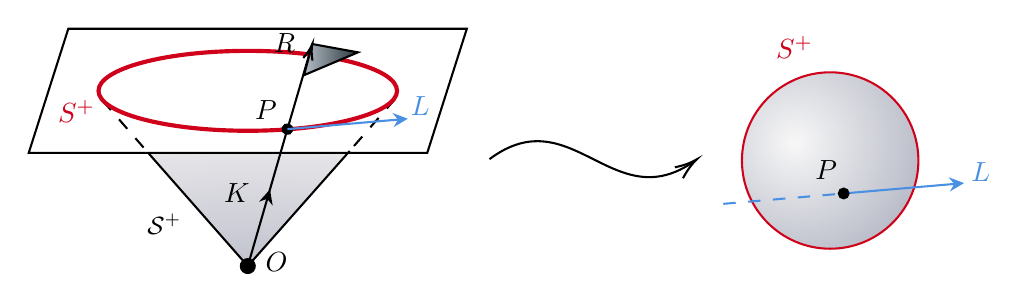
\begin{tikzpicture}[x=0.75pt,y=0.75pt,yscale=-1,xscale=1]
	%uncomment if require: \path (0,137); %set diagram left start at 0, and has height of 137
	
	%Shape: Triangle [id:dp18085529825630564] 
	\draw  [draw opacity=0][shading=_4ys9j1xwk,_xfijtitct] (203.92,121.29) -- (276.42,37.67) -- (131.41,37.67) -- cycle ;
	%Shape: Parallelogram [id:dp9228773357244249] 
	\draw  [fill={rgb, 255:red, 255; green, 255; blue, 255 }  ,fill opacity=1 ] (117.45,6.93) -- (309.46,6.93) -- (290.38,66.78) -- (98.37,66.78) -- cycle ;
	%Straight Lines [id:da7856751732458289] 
	\draw [shading=_pi2xaa4p6,_34dxukbo6]   (203.92,121.29) -- (156.01,66.83) ;
	%Straight Lines [id:da530742601835525] 
	\draw [shading=_2xbmbn3l0,_gw9u3nn4y]   (203.92,121.29) -- (253.01,65.83) ;
	\draw [shift={(203.92,121.29)}, rotate = 311.51] [color={rgb, 255:red, 0; green, 0; blue, 0 }  ][fill={rgb, 255:red, 0; green, 0; blue, 0 }  ][line width=0.75]      (0, 0) circle [x radius= 3.35, y radius= 3.35]   ;
	%Straight Lines [id:da4568538254779688] 
	\draw  [dash pattern={on 4.5pt off 4.5pt}]  (134.01,41.57) -- (156.01,66.83) ;
	%Straight Lines [id:da7131966021543883] 
	\draw  [dash pattern={on 4.5pt off 4.5pt}]  (274.83,40.85) -- (253.01,65.83) ;
	%Shape: Ellipse [id:dp8890884080819843] 
	\draw  [color={rgb, 255:red, 208; green, 2; blue, 27 }  ,draw opacity=1 ][line width=1.5]  (132,36.85) .. controls (132,26.22) and (164.2,17.6) .. (203.92,17.6) .. controls (243.64,17.6) and (275.83,26.22) .. (275.83,36.85) .. controls (275.83,47.49) and (243.64,56.1) .. (203.92,56.1) .. controls (164.2,56.1) and (132,47.49) .. (132,36.85) -- cycle ;
	%Straight Lines [id:da09373596447493804] 
	\draw    (223.01,55.31) -- (203.92,121.29) ;
	\draw [shift={(214.6,84.36)}, rotate = 106.14] [fill={rgb, 255:red, 0; green, 0; blue, 0 }  ][line width=0.08]  [draw opacity=0] (7.14,-3.43) -- (0,0) -- (7.14,3.43) -- (4.74,0) -- cycle    ;
	%Shape: Polygon [id:ds8121831694427222] 
	\path  [shading=_o1fem7bmr,_9byeair1q] (257.01,18.31) -- (231.01,29.31) -- (235.01,14.31) -- cycle ; % for fading 
	\draw   (257.01,18.31) -- (231.01,29.31) -- (235.01,14.31) -- cycle ; % for border 
	
	%Straight Lines [id:da8477468495579272] 
	\draw    (223.01,55.31) -- (234.44,16.23) ;
	\draw [shift={(235.01,14.31)}, rotate = 106.31] [color={rgb, 255:red, 0; green, 0; blue, 0 }  ][line width=0.75]    (7.65,-2.3) .. controls (4.86,-0.97) and (2.31,-0.21) .. (0,0) .. controls (2.31,0.21) and (4.86,0.98) .. (7.65,2.3)   ;
	\draw [shift={(223.01,55.31)}, rotate = 286.31] [color={rgb, 255:red, 0; green, 0; blue, 0 }  ][fill={rgb, 255:red, 0; green, 0; blue, 0 }  ][line width=0.75]      (0, 0) circle [x radius= 2.34, y radius= 2.34]   ;
	%Straight Lines [id:da15925016913815626] 
	\draw [color={rgb, 255:red, 74; green, 144; blue, 226 }  ,draw opacity=1 ]   (278.02,50.57) -- (223.01,55.31) ;
	\draw [shift={(281.01,50.31)}, rotate = 175.07] [fill={rgb, 255:red, 74; green, 144; blue, 226 }  ,fill opacity=1 ][line width=0.08]  [draw opacity=0] (7.14,-3.43) -- (0,0) -- (7.14,3.43) -- (4.74,0) -- cycle    ;
	%Curve Lines [id:da02129065464097457] 
	\draw    (320.38,69.78) .. controls (359.98,40.08) and (379.98,98.59) .. (419.19,70.65) ;
	\draw [shift={(420.38,69.78)}, rotate = 143.13] [color={rgb, 255:red, 0; green, 0; blue, 0 }  ][line width=0.75]    (10.93,-3.29) .. controls (6.95,-1.4) and (3.31,-0.3) .. (0,0) .. controls (3.31,0.3) and (6.95,1.4) .. (10.93,3.29)   ;
	%Shape: Circle [id:dp7494161810872726] 
	\path  [shading=_31p2pzfdp,_echxgy7iy] (442,70.43) .. controls (442,46.96) and (461.03,27.93) .. (484.5,27.93) .. controls (507.98,27.93) and (527.01,46.96) .. (527.01,70.43) .. controls (527.01,93.9) and (507.98,112.93) .. (484.5,112.93) .. controls (461.03,112.93) and (442,93.9) .. (442,70.43) -- cycle ; % for fading 
	\draw  [color={rgb, 255:red, 208; green, 2; blue, 27 }  ,draw opacity=1 ] (442,70.43) .. controls (442,46.96) and (461.03,27.93) .. (484.5,27.93) .. controls (507.98,27.93) and (527.01,46.96) .. (527.01,70.43) .. controls (527.01,93.9) and (507.98,112.93) .. (484.5,112.93) .. controls (461.03,112.93) and (442,93.9) .. (442,70.43) -- cycle ; % for border 
	
	%Straight Lines [id:da855599687264156] 
	\draw [color={rgb, 255:red, 74; green, 144; blue, 226 }  ,draw opacity=1 ]   (546.02,81.57) -- (491.01,86.31) ;
	\draw [shift={(549.01,81.31)}, rotate = 175.07] [fill={rgb, 255:red, 74; green, 144; blue, 226 }  ,fill opacity=1 ][line width=0.08]  [draw opacity=0] (7.14,-3.43) -- (0,0) -- (7.14,3.43) -- (4.74,0) -- cycle    ;
	%Straight Lines [id:da2554725584191] 
	\draw    (491.01,86.31) ;
	\draw [shift={(491.01,86.31)}, rotate = 0] [color={rgb, 255:red, 0; green, 0; blue, 0 }  ][fill={rgb, 255:red, 0; green, 0; blue, 0 }  ][line width=0.75]      (0, 0) circle [x radius= 2.34, y radius= 2.34]   ;
	%Straight Lines [id:da514198553655629] 
	\draw [color={rgb, 255:red, 74; green, 144; blue, 226 }  ,draw opacity=1 ] [dash pattern={on 4.5pt off 4.5pt}]  (433.01,91.31) -- (491.01,86.31) ;
	
	
	% Text Node
	\draw (211,113.5) node [anchor=north west][inner sep=0.75pt]    {$O$};
	% Text Node
	\draw (154,94.5) node [anchor=north west][inner sep=0.75pt]  [font=\small]  {$\mathcal{S}^{+}$};
	% Text Node
	\draw (111,40) node [anchor=north west][inner sep=0.75pt]  [color={rgb, 255:red, 208; green, 2; blue, 27 }  ,opacity=1 ]  {$S^{+}$};
	% Text Node
	\draw (205.92,39.85) node [anchor=north west][inner sep=0.75pt]    {$P$};
	% Text Node
	\draw (191,80) node [anchor=north west][inner sep=0.75pt]    {$\boldsymbol{K}$};
	% Text Node
	\draw (281,38) node [anchor=north west][inner sep=0.75pt]  [color={rgb, 255:red, 74; green, 144; blue, 226 }  ,opacity=1 ]  {$\boldsymbol{L}$};
	% Text Node
	\draw (215,7.94) node [anchor=north west][inner sep=0.75pt]    {$R$};
	% Text Node
	\draw (551,70) node [anchor=north west][inner sep=0.75pt]  [color={rgb, 255:red, 74; green, 144; blue, 226 }  ,opacity=1 ]  {$\boldsymbol{L}$};
	% Text Node
	\draw (475.92,68.85) node [anchor=north west][inner sep=0.75pt]    {$P$};
	% Text Node
	\draw (457,9) node [anchor=north west][inner sep=0.75pt]  [color={rgb, 255:red, 208; green, 2; blue, 27 }  ,opacity=1 ]  {$S^{+}$};
	
	
\end{tikzpicture}